\section{}
Consider the steady, incompressible, parallel laminar flow of a film of oil falling slowly down an infinite vertical wall.
The oil film thickness is $h$, and gravity acts in the negative $z$-direction. There is no applied pressure driving the flow,
the oil falls by gravity alone. Calculate the velocity fields in the oil film. The changes in the hydrostatic pressure of the
surrounding air can be neglected.   
\begin{figure}[h]
    \centering
    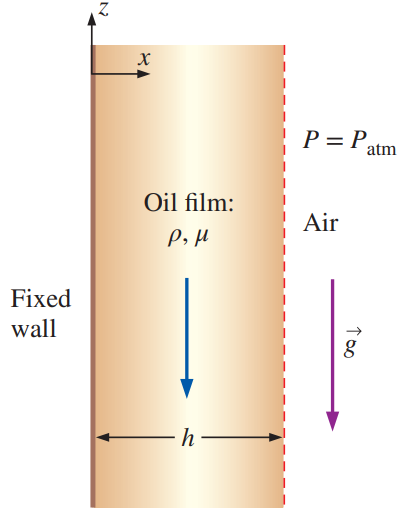
\includegraphics[width=0.3\linewidth]{Questions/Figures/Q3ProblemDiagram.png}
    \caption{Geometry of oil film falling by gravity down a vertical wall.}
    \label{fig:oil_film}
\end{figure}

\textbf{Solution:} \\
The continuity equation for incompressible flow is given by:
\begin{align*}
    \underbrace{\cancel{\frac{\partial u}{\partial x}}}_{\text{Parallel flow}} + \frac{\partial w}{\partial z} = 0 \\
    \frac{\partial w}{\partial z} = 0 \\
    w = f(x)
\end{align*}
The Navier-Stokes equation for incompressible, Newtonian fluids is given by:
\begin{align*}
    \rho \frac{D \vec{V}}{Dt} &= -\nabla P + \rho \vec{g} + \mu \nabla^2 \vec{V} \\
\end{align*}
Since the flow is steady, parallel, laminar, constant pressure, and gravity acts in the negative $z$-direction, the Navier-Stokes equation in the 
$z$-direction simplifies to:
\begin{align*}
    \rho \left(\underbrace{\cancel{\frac{\partial w}{\partial t}}}_{\text{Steady}} + \underbrace{\cancel{u \frac{\partial w}{\partial x}}}_{\text{u = 0}}
    + \underbrace{\cancel{w \frac{\partial w}{\partial z}}}_{\text{Continuity}}\right) 
    &= -\underbrace{\cancel{\frac{\partial P}{\partial z}}}_{\text{Constant}} + -\rho g_z
    + \mu \left(\frac{\partial^2 w}{\partial x^2} + \underbrace{\cancel{\frac{\partial^2 w}{\partial z^2}}}_{\text{Continuity}}\right) \\
    \implies \frac{\partial^2 w}{\partial x^2} &= \frac{\rho g_z}{\mu} 
\end{align*}
Since $w=f(x)$, a normal derivative can be used instead of a partial derivative:
\begin{align*}
    \frac{d^2 w}{d x^2} &= \frac{\rho g_z}{\mu} \\
    \implies w(x) &= \frac{\rho g_z}{2 \mu} x^2 + C_1 x + C_2
\end{align*}
Boundary conditions are to be specified. At $x=0$, along the wall, the no-slip condition applies, so $u = w = 0$. No shear at
the free surface, so $\frac{\partial w}{\partial z} = 0$ at $z=h$. Therefore,
\begin{align*}
    w(0) = C_2 \overset{\text{set}}{=} 0 \\
    \frac{\partial w}{\partial x}\bigg|_{x=h} = \frac{\rho g_z}{\mu} h + C_1 \overset{\text{set}}{=} 0 \\
    \implies C_1 = -\frac{\rho g_z}{\mu} h
\end{align*}
Therefore,
\begin{empheq}[box=\fbox]{align*}
    u &= 0 \\
    w(x) &= \frac{\rho g_z}{2 \mu} x^2 - \frac{\rho g_z h}{\mu} x
\end{empheq}